A \emph{scalar product} is a bilinear symmetric function $B: u,v\mapsto B(u,v)$, i.e.
\begin{equation}
\label{eq:scalar}
B(u,v)=B(v,u),
\quad
B(λ\cdot u + v,w) = λ\cdot B(u,w) + B(v,w)
\end{equation}
for all vectors $u,v,w$ and scalars $λ$.
All skew-symmetric bilinear functions on a two-dimensional vector space
form a three-dimensional vector space.

{\color{red} Write first a generic proposition that bilinearity implies quadraticity and choose particular $B= (.,.)$.}

Referring to \cref{fig:homot_norm} (left),
the trace of the scalar square is a constant:
\begin{equation}
\label{:norm2}
T_N |P|^2 = \frac{a^2 + b^2}{2}
\end{equation}

\begin{figure}
    \centering
    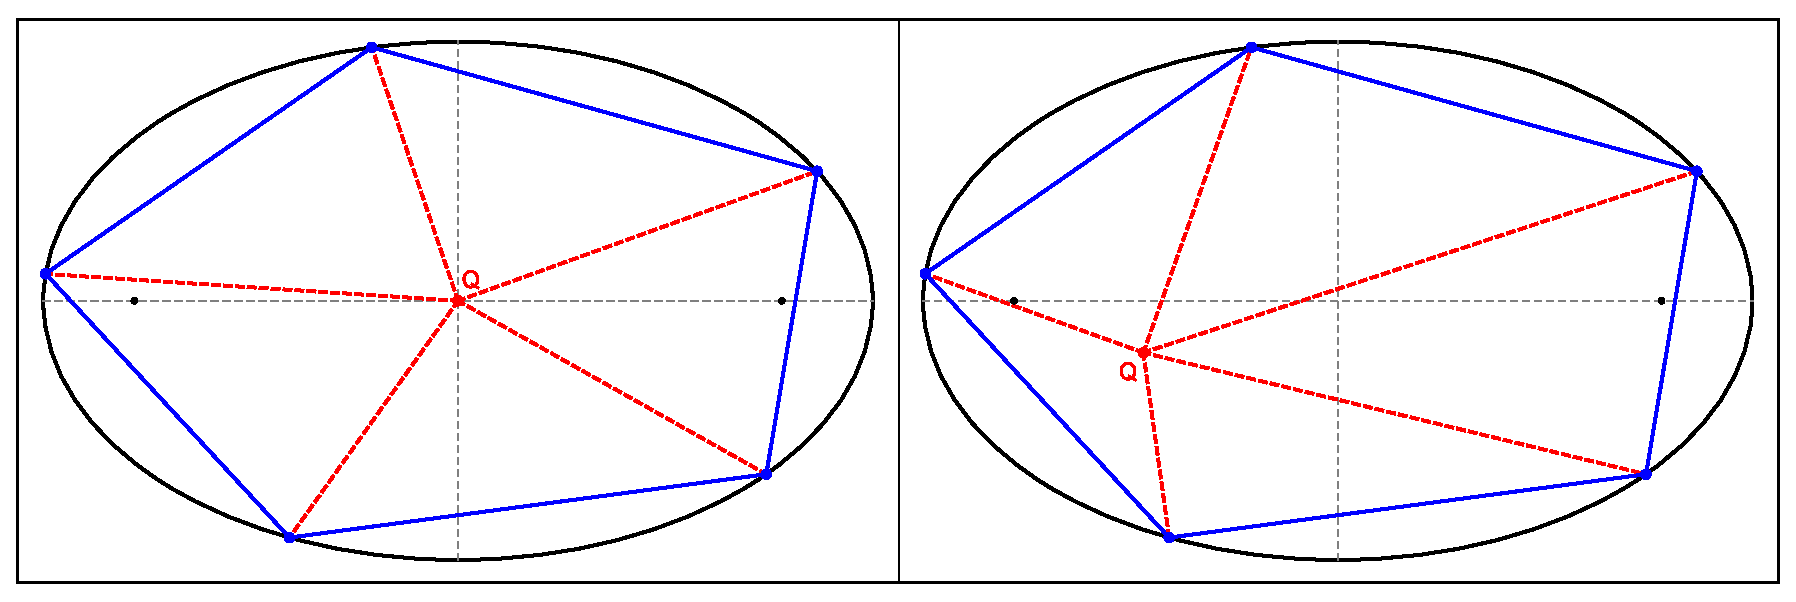
\includegraphics[width=\textwidth]{pics/0025_homot_norm_no_caustic.eps}
    \caption{\textbf{Left:} \cref{:norm2} states that the sum of squared norms of the vertices with respect to the center is invariant. \textbf{Right:} \cref{:p0} states that in fact the squared norms of vertices with respect to any point $P_0$ is invariant. \href{https://youtu.be/2PdsC3CcqaE}{Video}}.
    \label{fig:homot_norm}
\end{figure}

\begin{proof}
Apply \cref{:Laurent} with $f=(ax)^2+(by)^2$.
\end{proof}
\begin{remark}
For quadrangles this is known as
\href{https://en.wikipedia.org/wiki/Ellipse#Theorem_of_Apollonios_on_conjugate_diameters}{Theorem of Apollonios on conjugate diameters}.
\end{remark}

Let $s=|S(ρ(P)-P)|$ denote the sidelength,
then the trace $L_{2,N} := T_N s^2$ is a constant equal to
\begin{equation}
\label{:sqr_si}
T_N s^2 = \left[ 1-\cos \left(α\right) \right] \left( a^2+b^2 \right)
\end{equation}
\begin{proof}
Note that any rotation $ρ$ is linear, so coordinates of $ρ(P)-P$ are linear in $x,y$
and its scalar square is quadratic. Apply \cref{:Laurent}.
\end{proof}

Recall the Brocard angle $\omega$ of a triangle is given by $\cot\omega=L_{2,3}/(4A_3)$ \cite[Brocard Angle]{mw}. Then:

\begin{corollary}
Over $\FF$ with $N=3$, the Brocard angle $\omega$ is constant. 
\end{corollary}

Note: a well-known identity is that $\cot\omega=\cot\theta_1+\cot\theta_2+\cot\theta_3$.
\cref{:cot} is statement that this sum generalizes for $N>3$. 


Referring to \cref{fig:homot_norm}, the trace of the squared distance to any fixed point $Q$ is also constant:

\begin{equation}
\label{:p0}
T_N |P_k-Q|^2 = \frac{a^2 + b^2}{2} + |Q|^2
\end{equation}


